%% LaTeX2e Template by Stephen Iota (https://stepheniota.com/)
%% last updated: Feb. 2019
%% for papers
%\documentclass[aps,preprint,notitlepage]{revtex4-1}
%% https://www-d0.fnal.gov/Run2Physics/WWW/templates/revtex4.pdf
%% https://cdn.journals.aps.org/files/revtex/auguide4-1.pdf
%% ^^ revTeX4-1 class options

%% for other
\documentclass[11pt]{article}
\usepackage[margin=2cm]{geometry}
%%%%%%%%%%%%%%%%
%%% Packages %%%
%%%%%%%%%%%%%%%%

\usepackage[utf8]{inputenc}
\usepackage[noadjust]{cite}
\usepackage{lipsum}
\usepackage{amsmath}
\usepackage{amssymb}
\usepackage{amsfonts}
\usepackage{mathtools}
\usepackage{physics} %http://ftp.math.purdue.edu/mirrors/ctan.org/macros/latex/contrib/physics/physics.pdf
\usepackage[thinc]{esdiff} % easy derivatives
\usepackage{graphicx} % \includegraphics{ }
\usepackage[shortlabels]{enumitem} % change labels in enum/item environments
\usepackage[dvipsnames]{xcolor} % colored links=
%\usepackage{footmisc} % http://mirror.utexas.edu/ctan/macros/latex/contrib/footmisc/footmisc.pdf
%\usepackage[small]{titlesec} % [small,medium,big] << controls size of *section text
%\usepackage{fancyhdr} %http://tug.ctan.org/tex-archive/macros/latex/contrib/fancyhdr/fancyhdr.pdf
% always put this at the end
\usepackage[
	colorlinks=true,
	citecolor=NavyBlue!90!black,
	linkcolor=NavyBlue!75!black,
	urlcolor=green!50!black,
	hypertexnames=false]{hyperref}

 %%%%%%%%%%%%%%%%%%
 %% New Commands %%
 %%%%%%%%%%%%%%%%%%
\newcommand{\email}[1]{\texttt{\href{mailto:#1}{#1}}}
%\newcommand{\ave}[1]{$\langle #1 \rangle$}
\renewcommand{\d}[1]{\ensuremath{\operatorname{d}\!{#1}}}
%%%%%%%%%%%%%%%%%%
%% Front Matter %%
%%%%%%%%%%%%%%%%%%

%\pagenumbering{gobble} % no page numbers
\graphicspath{{figures/}} % set directory for figures
%\setcounter{section}{-1} % start with section 0


%%%%%%%%%%%%%
%%% Title %%%
%%%%%%%%%%%%%
\begin{document}



\begin{center}

\Large{\textsc{Statistical Mechanics}: \textbf{Problem Set 2}}
\end{center}
\vspace{.5mm}


%%%%%%%%%%
%% INFO %%
%%%%%%%%%%

\begin{tabular}{rl}
\textsc{Name}:
&
Stephen Iota (\email{siota001@ucr.edu})
\\
\textsc{Course}:
&
Physics 133 (Spring 2019), Prof.~Kuhlman
\\
\textsc{Date}:
&
\today
\end{tabular}
\vspace{2mm}
%%%%%%%%%%%%%%
%% PROBLEMS %%
%%%%%%%%%%%%%%

\noindent
Sethna problems 2.6, 3.5 and 3.9. Painstakingly typeset using \LaTeX. All final answers are \boxed{\text{boxed.}}

%%%%%%%%%%%%%%%%
%% Sethna 2.6 %%
%%%%%%%%%%%%%%%%
\section{Fourier and Green}

An initial denisty profile $\rho(x,t=0)$ is perturbed slightly from $\rho_0$. The density obeys the diffusion equation
$\pdv{\rho}{t} = D \pdv[2]{\rho}{x}$,
where $D = 0.001$ m/s$^2$.

\begin{figure}[h!]
\centering
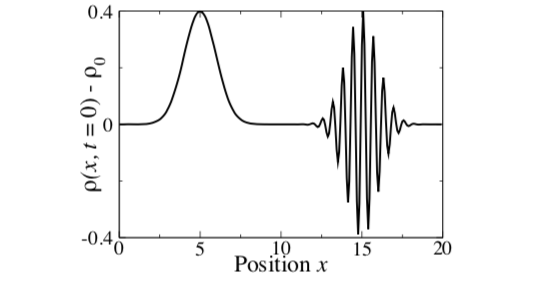
\includegraphics[width=.5\linewidth]{Pset2_Fig1}
\caption{Initial profile density deviation from average.\label{density}}
\end{figure}

\vspace{2mm}
\noindent
\textbf{(a) Fourier}
\textit{Consider just a cosine wave. If the intial wave were
$\rho_\text{cos}(x,0) = \cos{10x}$, what would it be at $t = 10s$?}

\vspace{2mm}
\noindent
\textbf{Solution:}
We can decompose $\rho$ into a superpostition of complex plane wave solutions using the Fourier method. We expect the solution to look like $\rho_\text{cos} = \rho_k e^{ikx}$.
We can superimpose all different wave vectors to get a general solution.
$$
\rho(x,t) = \frac{1}{2\pi} \int_{-\infty}^{\infty} \rho_k(0) e^{ikx} e^{-Dk^2t} \text{d}k
$$
where the coefficients $\rho_k(0)$ are the Fourier transform of the initial density profile
$$
\rho_k(0) = \int_{-\infty}^{\infty} \rho(x,0) e^{-ikx} \text{d}x
$$

Plugging in $\rho_\text{cos}(x,0) = \cos{10x}$, we get
\begin{align*}
\rho_k &= \int_{-\infty}^{\infty} \cos{10x} \ e^{-ikx} \text{d}x
\\
       &= \int_{-\infty}^{\infty} \frac{e^{i10x} + e^{-i10x}}{2} \ e^{-ikx} \text{d}x
\\
			 &= \frac{1}{2} \Big[ \delta(k-10) + \delta(k+10) \Big]
\end{align*}
So the initial distribution is composed of two frequencies.
Now we solve for the time evolution in position space.
\begin{align*}
\rho(x,t) &= \frac{1}{2\pi} \int_{-\infty}^{\infty} \frac{1}{2} \Big[ \delta(k-10) + \delta(k+10) \Big] e^{ikx} e^{-Dk^2t} \text{d}k
\\
          &= \frac{1}{4\pi} \int_{-\infty}^{\infty} \Big[ \delta(k-10)e^{ikx} e^{-Dk^2t} + \delta(k+10)e^{ikx} e^{-Dk^2t} \Big] \text{d}k
					\\
					&= \frac{1}{4\pi} \Big[ (e^{i10x} + e^{-i10x}) e^{-D100t}  \Big]
					\\
					&= \frac{1}{8\pi} \cos{10x} \ e^{-D100t}
\end{align*}
This is the general time evolution for $\rho_\text{cos}$. Solving for $t =0$ yields
\begin{align*}
\rho(x, t = 10s) &=  \frac{1}{8\pi} \cos{10x}\  e^{-(.001\cdot100\cdot10)}
\\
&=  \boxed{ \frac{1}{8\pi} \cos{10x}\  e^{-1}}
\end{align*}

\vspace{2mm}
\noindent
\textbf{(b) Green}
\textit{If a wave at some earlier time $-t_0$ were a $\delta$-function at $x = 0$, such that $\rho(x,-t_0) = \delta(x)$, what choice of time elapsed $t_0$ would yield a Gaussian $\rho(x,0) = \exp(-x^2/2)/\sqrt{2\pi}$ for the given diffusion constant $D$?}

\vspace{2mm}
\noindent
\textbf{Solution:}
We define Green's function $G(x,t)$ to be the time evolution of $G(x,t=-t_0) = \delta(x)$. We follow the same steps as in part a to solve for $G(x,t).$
\begin{align*}
G_k(-t_0) &= \int G(x,-t_0) e^{-ikx}\d{x}
\\
          &= \int \delta(x) e^{-ikx} = 1
\end{align*}
$G_k$ is independent of $k$. The time evolved Fourier transform is $G_k(t) = e^{-Dk^2(t+t_0)}.$
The time evolution in position space is
\begin{align*}
G(x,t) &= \frac{1}{2\pi} \int e^{ikx} G_k(-t_0) e^{-Dk^2(t+t_0)} \d{k}
\\
       &= \frac{1}{2\pi} \int e^{ikx} e^{-Dk^2(t+t_0)} \d{k}
\end{align*}
The answer to this integral is the well known Green's function for the diffusion equation
$$
G(x,t) = \frac{1}{\sqrt{4\pi D(t+t_0)}} e^{-x^2/4D(t+t_0)}
$$
We need to find a time $-t_0$ such that $G(x,0)$ looks like a Gaussian function centered about the origin for the given diffusion constant $D.$ By analysis, we see that a time of \boxed{t_0 = 500 \ \text{seconds}} will give a Gaussian at $t=0$.



\vspace{2mm}
\noindent
\textbf{(c) Pictures}
\textit{Now consider time evolution for the next ten seconds. The initial density profile $\rho(x,t = 0)$ is as shown in fig.~\ref{density}.
What figure represents the density at $t = 10s$?}



\vspace{2mm}
\noindent
\textbf{Solution:}
The density profile in fig.~\ref{density} is a Gaussian centered at $x=5$ on the left,
and a smooth envelope function multiplied by $\cos{10x}$ centered at $x=15$ on the right. From the previous two parts, we know that the Gaussian function takes a much longer time to diffuse that the cosine function. Thus, in 10 seconds, we expect the function on the left to remain fairly similar. The short wavelength parts of the cosine function will be suppressed.
We expect the distribution at $t = 10$ sec to look like \boxed{\text{fig.~\ref{10sec} (figure \textbf{E} from the text).}}

\begin{figure}[h!]
\centering
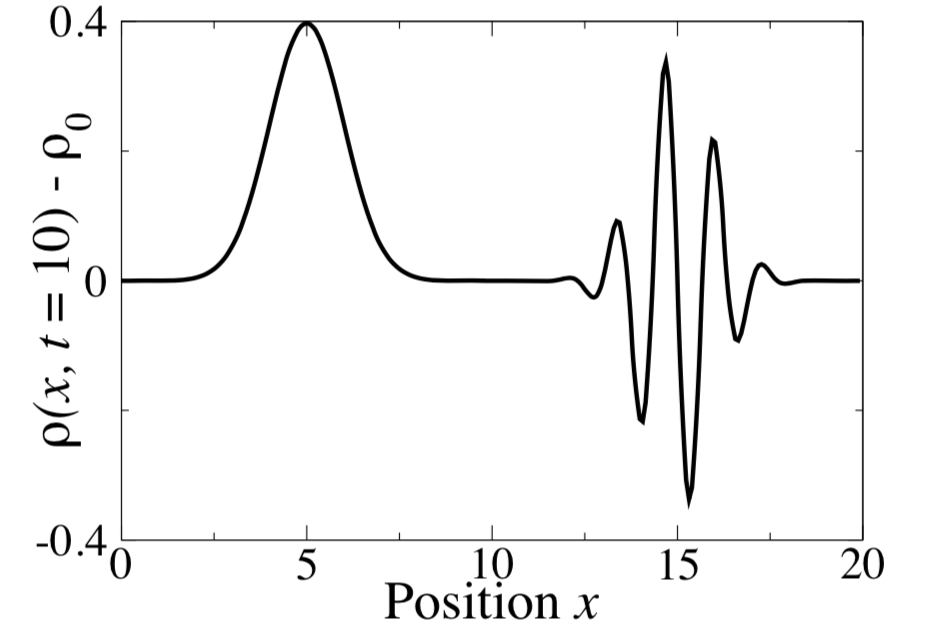
\includegraphics[width=.4\linewidth]{PSet2_Fig3}
\caption{Profile density at $t = 10$ seconds.}
\label{10sec}
\end{figure}

%%%%%%%%%%%%%%%%
%% Sentha 3.5 %%
%%%%%%%%%%%%%%%%
\section{Hard sphere gas}
A 2D $L \cross L$ box with hard walls contains a gas of $N$ hard disks of radius $r \ll L$, as shown in fig.~\ref{sphere}.
The disks are dilute; the summed area $N\pi r^2 \ll L^2$.
Let A be the effective area allowed for the disks in the box: $A = (L-2r)^2$.
\begin{figure}[h!]
	\centering
	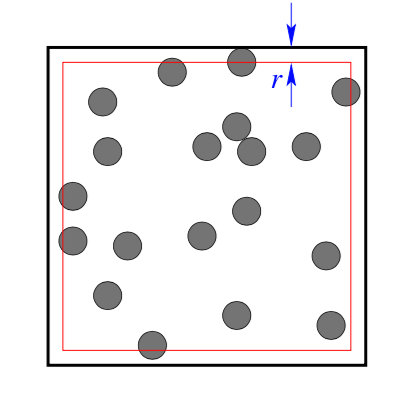
\includegraphics[width=.3\linewidth]{PSet2_Fig2}
	\caption{Hard sphere gas.}
	\label{sphere}
\end{figure}

\vspace{2mm}
\noindent
\textbf{(a)}
\textit{The area allowed for the second disk is approximately $A - \pi(2r)^2$.
What is the allowed 2N-dimensional volume in configuration space, of allowed zero-energy configurations of hard disks, in this dilute limit?}

\vspace{2mm}
\noindent
\textbf{Solution:}
For $N = 2$, $A_2 = A(A-4\pi r^2)$; for $N = 3$, $A_3 = A(A_2)(A_2 - 4\pi r^2)$, and so on. As $N$ increases, each disk will have a smaller area by $4\pi r^2$ than the previous disk.

$$
\boxed{A_N = \frac{1}{N!}\prod_{n = 0}^{N}A - n4\pi r^2}
$$


\vspace{2mm}
\noindent
\textbf{(b)}
\textit{
What is the configuration entropy for the hard disks?}

\vspace{2mm}
\noindent
\textbf{Solution:}
Let $S$ denote configuration entropy. Using answer from part a:

\begin{align*}
S &= k_B \log{A_N}
\\
  &= k_B \log{\Big( \frac{1}{N!}\prod_{n = 0}^{N}A - n4\pi r^2 \Big)}
	\\
	&= k_B \Big( -\log{N!} + \sum_{n = 1}^{N} \log{(A - (n-1)4\pi r^2)} \Big)
\end{align*}
where in the last step we changed the starting index.
In the dilute limit, $N 4\pi r^2 \ll A$. We taylor expand $\log{(A - n4\pi r^2)}$:
\begin{align*}
\log{(A - (n-1)4\pi r^2)} &= \log{A} + \log{(1 - (n-1)4\pi r^2/A)}
\\
&\approx \log{A} - (n-1)\frac{4\pi r^2}{A}
\end{align*}
Plugging in this approximation to the sum, we find a sum of the form $\sum_{n = 1}^{N} = N(N-1)/2$.
We use Stirling's approximation $\log{N!} \approx N \log{N} - N$.
\begin{align*}
S &= k_B \Bigg( - N \log{N} - N + \bigg( N\log{A} - \frac{N(N-1) 4\pi r^2}{2A} \bigg) \Bigg)
\end{align*}
Simplifying, we reach our result
$$
\boxed{S = N k_B \bigg( 1 + \log{\Big( \frac{A}{N} - \frac{4\pi r^2}{N}\frac{N - 1}{2} \Big)} \bigg)}
$$
where we might possibly be able to say $ \frac{4\pi r^2}{N}\frac{N - 1}{2}$ is about $2\pi r^2$.
%%%%%%%%%%%%%%%%
%% Sentha 3.9 %%
%%%%%%%%%%%%%%%%
\section{Gauss and Poisson}
Calculate the probability of having $n$ particles in a subvolume $V$, for a box with total volume $KV$ and a total number of particles $T = KN_0$.

\vspace{2mm}
\noindent
\textbf{(a)}
\textit{Find the exact formula for this probability; $n$ particles fall in the subvolume $V$, with a total of $T$ particles in $KV$.}

\vspace{2mm}
\noindent
\textbf{Solution:}
Suppose $n$ particles are in subvolume $V$ and $T - n$ particles are outside of $V$, in subvolume $(K-1)V$, where the total volume is $KV$.
In configuration space, the available volume is $V^n ((K - 1)V)^{T - n} = V^T (K-1)^{T - n}$, and the total volume is $(KV)^T$. The probability is given by the ratio of these two volumes, where we need to be mindful about the different ways to pick the $n$ particles. The total probability is given by:
\begin{align*}
P(n) &= \binom{T}{n} \frac{(K - 1)^{T - n}}{K^T}
\\
     &= \boxed{\frac{T!}{n!(T - n)!} \frac{(K - 1)^{T - n}}{K^T}}
\end{align*}


\vspace{2mm}
\noindent
\textbf{(b)}
\textit{
Show that the Poisson distribution in normalized: $\sum_n \rho_n = 1$.
Calculate the mean of the distribution $\langle n \rangle$ in terms of $a$. Calculate the variance $\langle(n - \langle n\rangle)^2\rangle$.}

\vspace{2mm}
\noindent
\textbf{Solution:}
For normalization:
\begin{align*}
\sum_{n=0}^{\infty} \rho_n &= \exp{-a} \sum_{n=0}^{\infty} \frac{a^n}{n!}
\\
&= \exp{-a} \exp{a}
\\
&= \boxed{1}
\end{align*}
For mean of Poisson distribution:
\begin{align*}
\langle n \rangle &= \sum_{n=0}^{\infty} n \frac{a^n}{n!} e^{-a}
\\
&= \sum_{n=1}^{\infty} n \frac{a^n}{n!} e^{-a}
\\
&= \sum_{n=1}^{\infty} \frac{aa^{n-1}}{(n-1)!} e^{-a}
\\
&= a \sum_{n=0}^{\infty} \frac{a^n}{n!} e^{-a}
\\
&= a \sum_{n=0}^{\infty} \frac{a^n}{n!} e^{-a}
\\
&= a \sum_{n=0}^{\infty} \rho_n
\end{align*}
which is equal to $\boxed{a}$ because the distribution is normalized.
For the variace, we have
$
\langle(n - \langle n\rangle)^2\rangle = \langle n^2 \rangle - \langle n \rangle^2
$.
\begin{align*}
\langle n\rangle)^2 &= \sum_{n=0}^{\infty} n^2 \frac{a^n}{n!} e^{-a}
\\
&= a \sum_{n=0}^{\infty} (n+1)\rho_n
\\
&= a \langle n+1 \rangle
\\
&= a^2 + a
\end{align*}
This gives us a variance of $(a^2 + a) - (a^2) = \boxed{a}$.


\vspace{2mm}
\noindent
\textbf{(c)}
\textit{As $K \rightarrow \infty$, show that the probability that $n$ particles fall in the subvolume $V$ has the Poisson distribution $\rho_n = a^n e^{-a}/n!$. What is $a$?}

\vspace{2mm}
\noindent
\textbf{Solution:}
Recall the answer to part a:
$$
P(n) = \frac{T!}{n!(T - n)!} \frac{(K - 1)^{T - n}}{K^T}
$$
As we let $K \text{and} T \rightarrow \infty, \ (1 - 1/K)^(T-n) \approx e^{\frac{T}{K}}.$ Also $T! \approx (T/e)^T$. We simplify:

\begin{align*}
\frac{T!}{n!(T - n)!}
&\approx \frac{(T/e)^T}{((T-n)/e)^{T-n}}
\\
&= \Big(\frac{T-n}{T}\Big)^{n-T}  \ \Big(\frac{T}{e}\Big) ^n
\\
&\approx e^{\frac{n}{T}(T-n)} \Big(\frac{T}{e}\Big)^N
\\
&\approx T^n
\end{align*}
The final result is a Poisson distribution where $a = T/K.$
$$
\boxed{
P(n) = \frac{(T/K)^n}{n!} e^{-T/K}
}
$$

\end{document}
